\documentclass[conference]{IEEEtran}
\IEEEoverridecommandlockouts
\usepackage{cite}
\usepackage{amsmath,amssymb,amsfonts}
\usepackage{graphicx}
\usepackage{textcomp}
\usepackage{booktabs}
\usepackage{url}

\begin{document}

\title{On-Device Acoustic Gunshot Detection: Data Cleaning, Model Comparison, and a One-Bit Edge Alert}

\author{
\IEEEauthorblockN{1\textsuperscript{st} Jeevant Sharma}
\IEEEauthorblockA{\textit{Department of Computer Science and Engineering} \\
\textit{Indian Institute of Information Technology, Surat}\\
Surat, India \\
jeevant.sharma@iiitsurat.ac.in}
\and
\IEEEauthorblockN{2\textsuperscript{nd} Deepesh Dangi}
\IEEEauthorblockA{\textit{Department of Computer Science and Engineering} \\
\textit{Indian Institute of Information Technology, Surat}\\
Surat, India \\
deepesh.dangi@iiitsurat.ac.in}
\and
\IEEEauthorblockN{3\textsuperscript{rd} Dr. Kaustubh Dhondge}
\IEEEauthorblockA{\textit{Department of Computer Science and Engineering} \\
\textit{Indian Institute of Information Technology, Surat}\\
Surat, India \\
kaustubh@iiitsurat.ac.in}
}

\maketitle

\begin{abstract}
Acoustic gunshot detection on low-cost embedded edge platforms presents physical challenges including transducer domain shift, diaphragm saturation at high sound pressure levels, electrical DC voltage rail drift, thermal ADC hiss amplification, and false triggers from percussive imposter sounds. This paper reports a detector designed for deployment on an Arduino Nano 33 BLE Sense. Training and evaluation were conducted on a host PC. Edge timing was profiled on a virtual machine throttled to 45--50\% CPU utilization to approximate a Raspberry Pi~4. Audio data was cleaned using librosa at window lengths of 250\,ms, 500\,ms, and 1\,s. The operational window is 750\,ms, since a 250\,ms cut removes the reverberation decay that distinguishes a gunshot from a percussive knock. Classical classifiers (logistic regression, SVM, random forest) achieved 99--100\% accuracy on balanced hold-out files but failed on live microphone input. Five neural architectures were trained and evaluated. On a 1{,}442-clip balanced hold-out, three models exceed 99.5\% accuracy. On 300 unseen recordings, the best single-model sliding-window gunshot recall is 67\%, achieved by the Enhanced 2D CNN which executes in 0.09\,ms within a 123.6\,KB INT8 footprint. A three-model ensemble raises recall to 77\% within 715\,KB and 17\,ms combined. The proposed deployment architecture retains all audio on the sensor node, transmits only a single-bit detection flag (1~for gunshot, silence otherwise), and requires spatial consensus from multiple neighbouring nodes at the gateway before raising an alert.
\end{abstract}

\begin{IEEEkeywords}
Acoustic gunshot detection, edge inference, TinyML, PCEN, convolutional recurrent neural networks, Arduino Nano 33 BLE Sense.
\end{IEEEkeywords}

% ==============================================================================
\section{Introduction}
\label{sec:intro}

Firearm violence in urban environments demands rapid, automated detection and localization of gunshot events. Empirical studies indicate that a significant fraction of firearm discharges in affected neighbourhoods are never reported by witnesses. When reports are made, they are frequently delayed and spatially inaccurate. An automated acoustic sensing system deployed across a campus, urban block, or wildlife sanctuary can detect the event within seconds and dispatch emergency response to the precise location.

Dense urban environments present the hardest deployment scenario due to continuous traffic, construction, and festival fireworks. Institutional campuses---colleges, schools, government perimeters---offer a more controlled starting point with known site geometry and reduced ambient impulsive noise.

The target deployment platform for this work is the Arduino Nano 33 BLE Sense. The node must execute inference locally without streaming microphone audio to any external server, preserving civilian privacy. This paper covers the stages preceding physical deployment: model training on a PC, conversion from Keras (\texttt{.h5}) to TensorFlow Lite (\texttt{.tflite}), INT8 quantization, and latency profiling on a virtual Raspberry Pi. The deployment design---duty-cycled sleep, one-bit radio transmission, and multi-node spatial consensus at a gateway---is specified in Section~\ref{sec:conclusion} as the immediate next phase.

The remainder of this paper is organized as follows. Section~\ref{sec:related} reviews related work. Section~\ref{sec:method} describes the data pipeline, feature extraction, and model architectures. Section~\ref{sec:setup} defines evaluation protocols and metrics. Section~\ref{sec:results} presents experimental results. Section~\ref{sec:conclusion} discusses conclusions and planned hardware deployment.

% ==============================================================================
\section{Related Work}
\label{sec:related}

\subsection{Acoustic Gunshot Detection Systems}
Municipal acoustic surveillance systems have demonstrated the viability of city-scale gunshot detection. Open datasets such as the multi-firearm, multi-orientation recording set published in \emph{Data in Brief}~\cite{dib2023} provide calibrated multi-caliber recordings for research use. These files, along with other firearm and ambient recordings, form part of our training corpus. Commercial systems validate the concept but typically require continuous audio streaming to centralized cloud infrastructure, raising bandwidth costs and civilian privacy concerns that are incompatible with campus-scale edge deployment.

\subsection{Per-Channel Energy Normalization}
Per-channel energy normalization (PCEN) was proposed for bioacoustic sound event detection~\cite{lostanlen2019}. PCEN divides each frequency band by a smoothed running estimate of its own background energy, suppressing stationary noise (rain, wind, HVAC) while preserving sudden transient impulses. One of our models adopts this front-end. The network architecture, training data, and evaluation methodology are original to this work.

\subsection{TinyML and Edge Impulse}
Edge Impulse was used as a preliminary TinyML evaluation platform on an ARM Cortex-M4F target prior to our main TensorFlow-based models. MixUp regularization~\cite{zhang2018} and SpecAugment~\cite{park2019} are employed within the enhanced convolutional architectures.

% ==============================================================================
\section{Method}
\label{sec:method}

\subsection{Data Cleaning and Window Length Selection}
The raw data pool comprised approximately 80{,}000 audio files drawn from firearm recording datasets and extended ambient recordings. Cleaning was performed using librosa. Approximately 1{,}000 to 5{,}000 clips were manually audited in iterative listening cycles until the retained clips met quality requirements.

Candidate window lengths of 250\,ms, 500\,ms, and 1\,s were evaluated. The muzzle blast attack phase lasts only a few milliseconds, but the environmental reverberation decay that follows persists for several hundred milliseconds. A 250\,ms window retains the attack but discards most of the decay, causing gunshots and percussive knocks to become spectrally similar. The neural models use a \textbf{750\,ms window} (16{,}537 samples at 22{,}050\,Hz). On the live inference path, consecutive windows overlap by 75\% (hop of 187.5\,ms) to ensure that any transient event falls fully within at least one analysis frame.

Negative-class clips containing sharp percussive transients (with crest factor and attack energy matching gunshot profiles) were removed to prevent label contamination. Class balance was systematically varied: initial 1:1 ratios produced the reported 99--100\% classical accuracy figures, while later training used 1:10 to 1:50 negative-heavy ratios to better approximate continuous monitoring conditions.

\subsection{Classical Machine Learning Baseline}
Logistic regression was first employed to assess whether handcrafted spectral features could achieve class separation. An SVM with RBF kernel and a random forest (100 estimators) were subsequently trained on MFCC and related spectral summaries at class ratios from 1:1 to 1:10.

On held-out files from the cleaned pool, several configurations achieved 99--100\% accuracy. On live microphone input, these classifiers failed. Computing static MFCC summaries requires averaging spectral frames across the temporal window, which smooths out the sub-3\,ms shockwave attack---the primary distinguishing signature---into a blurred frequency envelope. Everyday sounds with similar spectral centroids (cutlery, vehicle brakes, keys) produced continuous false alarms. These results confirmed that static feature engineering is inadequate for impulsive acoustic events.

\subsection{Edge Impulse Evaluation}
Five Edge Impulse configurations were evaluated on an ARM Cortex-M4F target (64\,MHz, 256\,KB SRAM) prior to the main TensorFlow models. Table~\ref{tab:edgeimpulse} summarizes the progression.

\begin{table}[!t]
\centering
\caption{Edge Impulse experiment progression on ARM Cortex-M4F.}
\label{tab:edgeimpulse}
\footnotesize
\begin{tabular}{llcccl}
\toprule
\textbf{Exp} & \textbf{Features} & \textbf{Val.} & \textbf{Lat.} & \textbf{Flash} & \textbf{Live Result} \\
\midrule
1 & 13 MFCCs, 1D & 99.4\% & 1\,ms & 45\,KB & 70\% false alarms \\
2 & MFCC+Anomaly & 99.4\% & 2\,ms & 45\,KB & 98\% flagged \\
3 & MFE, 1D CNN & 98.8\% & 12\,ms & 47\,KB & 50\% false alarms \\
4 & MFE, 2D CNN & 99.6\% & 167\,ms & 52\,KB & 76--80\% reject \\
5 & MFE+Anomaly & 99.7\% & 167\,ms & 52\,KB & Best rejection \\
\bottomrule
\end{tabular}
\end{table}

The MFCC-based 1D CNN (Experiment~1) achieved 99.4\% validation accuracy but flagged 33 of 47 ambient windows as gunshots on live audio---a 70.2\% false alarm rate. This occurs because MFCC coefficients average out the shockwave transient, making speech formants and muzzle blasts spectrally similar. The 2D CNN operating on MFE spectrograms (Experiment~4) was the first configuration to successfully reject wind (75.8\%) and thunder (80.0\%) imposters. These results motivated the transition to custom spectrogram-based CNN architectures.

\subsection{Neural Model Architectures}
Five neural models share the 750\,ms conditioning front-end. The device-level preprocessing subtracts the sample mean to remove DC bias from the microphone supply rail, and applies peak normalization only when window RMS exceeds a threshold of 0.005 to prevent amplification of ADC thermal noise in quiet conditions.

\begin{table}[!t]
\centering
\caption{Neural model specifications.}
\label{tab:models}
\footnotesize
\begin{tabular}{lrr}
\toprule
\textbf{Model} & \textbf{Parameters} & \textbf{INT8 Size} \\
\midrule
Baseline 1D CNN (raw waveform) & 92{,}513 & 112.5\,KB \\
Baseline 2D CNN (log-mel) & 249{,}985 & 259.9\,KB \\
Enhanced 1D CNN (dual-head) & 96{,}674 & 118.5\,KB \\
Enhanced 2D CNN (log-mel) & 110{,}594 & 123.6\,KB \\
CRNN-PCEN (Bi-GRU) & 397{,}842 & 478.9\,KB \\
\bottomrule
\end{tabular}
\end{table}

\textbf{Baseline 1D CNN} (92{,}513 parameters): Operates directly on 16{,}537 raw audio samples. The first convolutional layer uses an 80-sample kernel ($\approx$3.6\,ms at 22{,}050\,Hz), spanning the duration of a typical shockwave attack. This layer functions as a learnable bank of 32~FIR filters tuned to impulsive rise times. Achieved 99.7\% accuracy on clean hold-out data; recall dropped to 30\% on unseen microphones due to acoustic domain collapse.

\textbf{Baseline 2D CNN} (249{,}985 parameters): Transforms audio into a 64-band log-mel spectrogram over 130~time frames. An early training run fed unnormalized decibel values ($-80$ to $0$\,dB) into ReLU activations, which output zero across the entire input range. This ``Dying ReLU'' collapse produced 0\% recall (721 false negatives on the hold-out). Rescaling inputs to $[0,1]$ via $(S_{\mathrm{dB}}+80)/80$ resolved the issue, restoring convergence to 99.86\% ROC-AUC.

\textbf{Enhanced Models} (dual-head): Incorporate MixUp augmentation ($\lambda \sim \mathrm{Beta}(0.3, 0.3)$), SpecAugment on the 2D path, and a secondary anomaly-score head. The Enhanced 1D variant was trained with heavy false-negative penalties. After INT8 quantization, this model predicts gunshot on every input including silence---a documented quantization failure caused by weight saturation in narrow-dynamic-range dilated 1D convolutions. The Enhanced 2D variant quantized successfully and serves as the primary production model.

\textbf{CRNN-PCEN} (397{,}842 parameters): Replaces the static log-mel front-end with PCEN~\cite{lostanlen2019}:
\begin{equation}
P[f,t] = \left( \frac{S[f,t]}{(\epsilon + M[f,t])^{\alpha}} + \delta \right)^{r} - \delta^{r}
\label{eq:pcen}
\end{equation}
where $M[f,t]$ is a causal background estimate via a first-order IIR smoother. With $\alpha \approx 0.98$, stationary noise collapses toward unity ($S_0^{0.02} \approx 1.0$) while transient impulses are preserved. Spatial features are processed by a bidirectional GRU ($2 \times 64$ units) that tracks the shockwave onset forward and the reverberation decay backward.

\begin{figure}[!t]
\centering
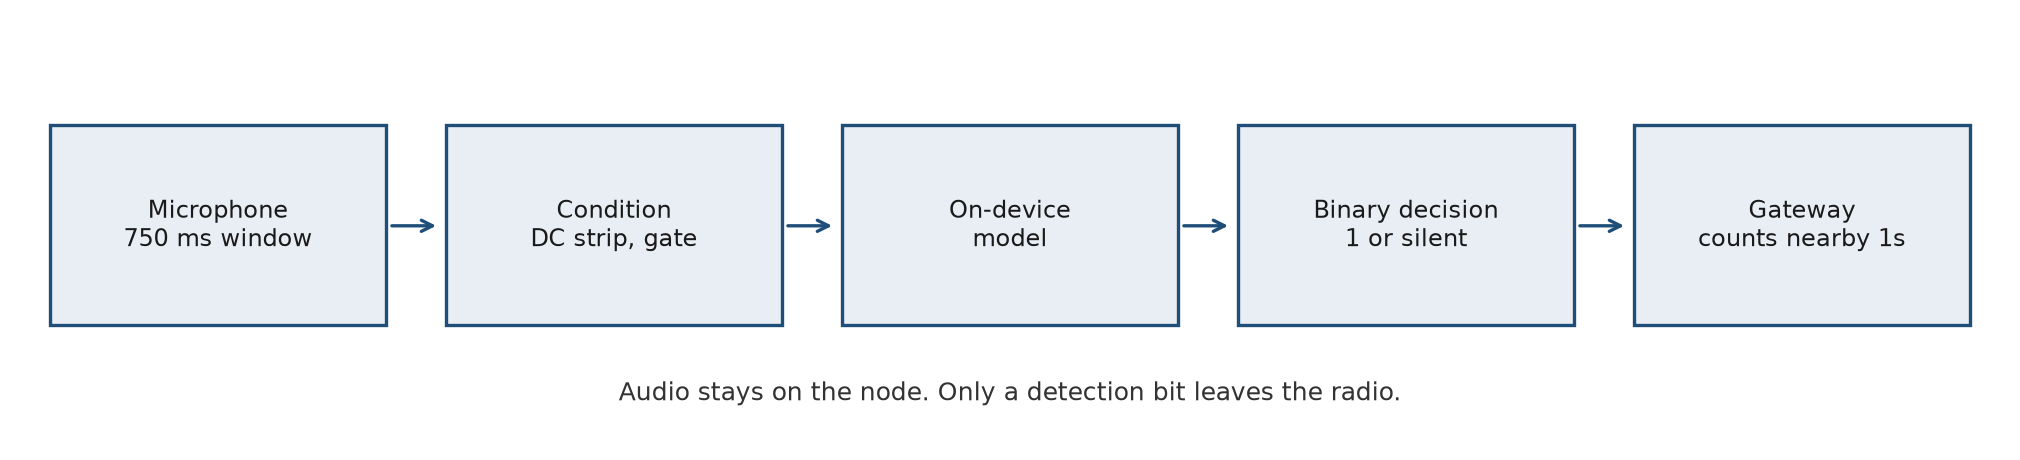
\includegraphics[width=\columnwidth]{figures/fig1_edge_pipeline.png}
\caption{Edge inference pipeline. Audio remains on the sensor node. Only a detection bit reaches the gateway.}
\label{fig:pipeline}
\end{figure}

% ==============================================================================
\section{Experimental Setup and Metrics}
\label{sec:setup}

\subsection{Evaluation Platforms}
All neural model evaluations used exported INT8 TensorFlow Lite models. Latency profiling was conducted on a VirtualBox virtual machine configured with four virtual CPUs at 45--50\% execution cap and 2\,GB RAM, approximating the computational throughput of a Raspberry Pi~4 (quad-core ARM Cortex-A72 at 1.5\,GHz). Each model was timed over 100 inference iterations.

\subsection{Evaluation Datasets}
Three evaluation sets were used:
\begin{itemize}
    \item \textbf{Balanced hold-out}: 1{,}442 clips of 750\,ms (721 gunshot, 721 non-gunshot) from the cleaned training pool.
    \item \textbf{75-clip external}: 20 firearms, 20 imposters, 35 ambient tracks from community sources. No overlap with training data.
    \item \textbf{300-clip unseen benchmark}: 100 real gunshots, 100 ambient non-gunshots, 100 hard imposters (fireworks, firecrackers, door slams, explosions, thunderclaps). No overlap with training data.
\end{itemize}

\subsection{Metrics}
\begin{itemize}
    \item \textbf{Gunshot recall}: Fraction of real gunshot files exceeding the decision threshold.
    \item \textbf{Ambient specificity}: Fraction of ambient files remaining below the threshold.
    \item \textbf{Imposter rejection}: Fraction of percussive imposter files remaining below the threshold.
    \item \textbf{Latency}: Time to score one 750\,ms window. The real-time constraint is the 187.5\,ms hop interval.
\end{itemize}
Decision threshold is 0.50 unless stated otherwise. Two scoring modes are reported: \textbf{peak-centered} (one 750\,ms slice around the loudest sample) and \textbf{sliding-window} (stepping across the full recording with 75\% overlap).

% ==============================================================================
\section{Results}
\label{sec:results}

\subsection{Balanced Hold-Out (1{,}442 Clips)}
Table~\ref{tab:holdout} verifies training convergence. Three models exceed 99.5\% accuracy on the balanced set. The broken 2D row is the unscaled-decibel checkpoint (721~false negatives). The Enhanced~1D row reflects the quantization failure (positive prediction on every input).

\begin{table}[!t]
\centering
\caption{Balanced hold-out results (1{,}442 clips, $\tau = 0.50$).}
\label{tab:holdout}
\footnotesize
\begin{tabular}{lccc}
\toprule
\textbf{Model} & \textbf{Accuracy} & \textbf{Recall} & \textbf{FP} \\
\midrule
Baseline 1D CNN & 99.79\% & 99.72\% & 1 \\
CRNN-PCEN & 99.79\% & 99.72\% & 1 \\
Enhanced 2D CNN & 99.51\% & 99.58\% & 4 \\
2D CNN (unscaled dB) & 50.00\% & 0.00\% & 0 \\
Enhanced 1D CNN (INT8) & 50.00\% & 100\% & 721 \\
\bottomrule
\end{tabular}
\end{table}

\subsection{75-Clip External Recordings}
On 75 external recordings scored with sliding windows at 75\% overlap (Table~\ref{tab:external}), the Enhanced 2D CNN detected 17 of 20 gunshots while ignoring 33 of 35 ambient tracks. The CRNN-PCEN ignored all 35 ambient files with zero false alarms. The Baseline 1D CNN recall dropped from 99.7\% (hold-out) to 30\%, indicating memorization of training microphone waveforms. On a 35-window clapping file, the CRNN-PCEN triggered on 23 windows because PCEN amplifies any rapid non-stationary transient.

\begin{table}[!t]
\centering
\caption{75-clip external evaluation (sliding, $\tau = 0.50$).}
\label{tab:external}
\footnotesize
\begin{tabular}{lccc}
\toprule
\textbf{Model} & \textbf{Recall} & \textbf{Ambient} & \textbf{Imposter} \\
\midrule
Enhanced 2D CNN & 17/20 (85\%) & 33/35 (94\%) & 7/20 (35\%) \\
CRNN-PCEN & 12/20 (60\%) & 35/35 (100\%) & 8/20 (40\%) \\
Baseline 1D CNN & 6/20 (30\%) & 31/35 (89\%) & 11/20 (55\%) \\
\bottomrule
\end{tabular}
\end{table}

\begin{figure}[!t]
\centering
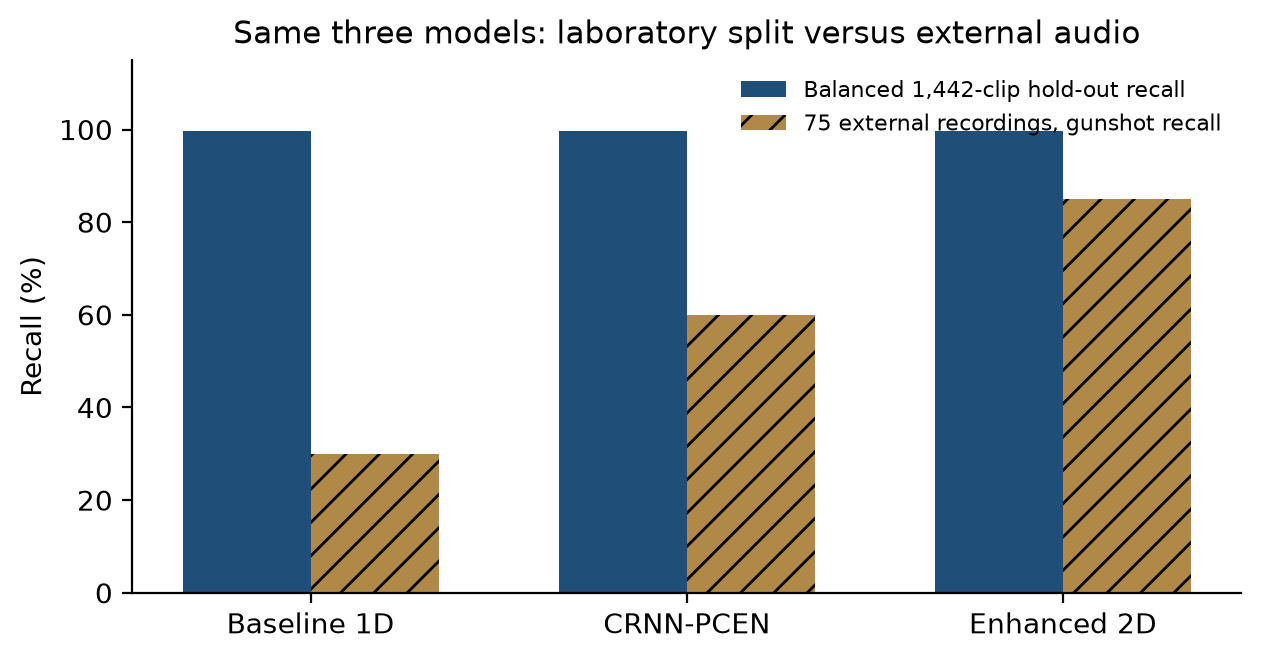
\includegraphics[width=\columnwidth]{figures/fig4_lab_vs_external.png}
\caption{Hold-out recall versus recall on 75 external recordings, illustrating acoustic domain shift.}
\label{fig:drop}
\end{figure}

\subsection{300-Clip Unseen Benchmark}
Tables~\ref{tab:slide} and~\ref{tab:peak} present the primary evaluation on 300 unseen clips using INT8 models at threshold 0.50 on the virtual Raspberry Pi.

\begin{table}[!t]
\centering
\caption{Sliding-window results (300 clips, $\tau = 0.50$).}
\label{tab:slide}
\footnotesize
\begin{tabular}{lccc}
\toprule
\textbf{Model} & \textbf{Recall} & \textbf{Amb. Spec.} & \textbf{Imp. Rej.} \\
\midrule
Baseline 1D CNN & 45\% & 85\% & 72\% \\
Baseline 2D CNN & 66\% & 88\% & 59\% \\
Enhanced 1D CNN$^*$ & 100\% & 0\% & 0\% \\
Enhanced 2D CNN & \textbf{67\%} & 82\% & 66\% \\
CRNN-PCEN & 57\% & 86\% & 61\% \\
\bottomrule
\multicolumn{4}{l}{\footnotesize $^*$INT8 quantization failure; predicts positive on all inputs.}
\end{tabular}
\end{table}

\begin{table}[!t]
\centering
\caption{Peak-centered results (300 clips, $\tau = 0.50$).}
\label{tab:peak}
\footnotesize
\begin{tabular}{lccc}
\toprule
\textbf{Model} & \textbf{Recall} & \textbf{Amb. Spec.} & \textbf{Imp. Rej.} \\
\midrule
Baseline 1D CNN & 30\% & 95\% & 84\% \\
Baseline 2D CNN & 45\% & 94\% & 77\% \\
Enhanced 1D CNN$^*$ & 100\% & 0\% & 0\% \\
Enhanced 2D CNN & 38\% & \textbf{99\%} & \textbf{89\%} \\
CRNN-PCEN & 33\% & 97\% & 85\% \\
\bottomrule
\multicolumn{4}{l}{\footnotesize $^*$INT8 quantization failure.}
\end{tabular}
\end{table}

\begin{figure}[!t]
\centering
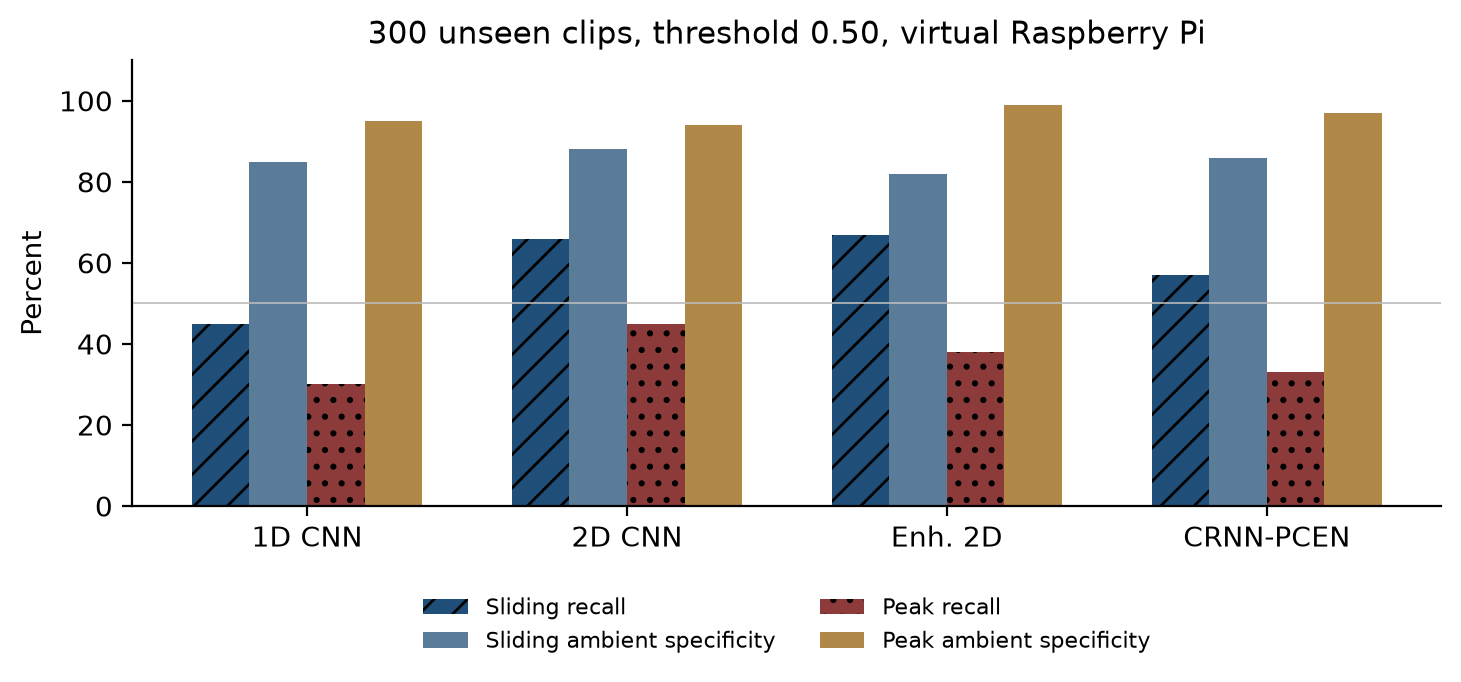
\includegraphics[width=\columnwidth]{figures/fig2_300clip_recall.png}
\caption{Sliding-window and peak-centered recall and specificity across 300 unseen clips.}
\label{fig:300}
\end{figure}

Sliding-window mode increases gunshot recall by 15 to 29 percentage points relative to peak-centered mode for all working models, at the cost of reduced specificity. Peak-centered mode achieves up to 99\% ambient specificity (Enhanced 2D CNN). This recall--specificity trade-off motivates the multi-model ensemble evaluated in Section~\ref{sec:ensemble}.

Cross-platform validation shows host-to-VM peak recall variance of 4--6 percentage points (e.g., Enhanced 2D CNN: 44.1\% host, 38.0\% VM), attributable to INT8 quantization rounding differences between x86 XNNPACK and ARM NEON kernels. Model ranking remains consistent across platforms.

\subsection{Latency Profiling}
Table~\ref{tab:latency} reports INT8 inference latency over 100 iterations on the throttled virtual machine. All models complete inference well within the 187.5\,ms real-time hop constraint.

\begin{table}[!t]
\centering
\caption{INT8 latency on the throttled virtual machine (100 iterations).}
\label{tab:latency}
\footnotesize
\begin{tabular}{lccc}
\toprule
\textbf{Model} & \textbf{INT8} & \textbf{Mean} & \textbf{Hop \%} \\
\midrule
Baseline 1D CNN & 112.5\,KB & 2.29\,ms & 1.2\% \\
Baseline 2D CNN & 259.9\,KB & 2.15\,ms & 1.2\% \\
Enhanced 1D CNN & 118.5\,KB & 2.69\,ms & 1.4\% \\
Enhanced 2D CNN & 123.6\,KB & \textbf{0.09\,ms} & \textbf{0.05\%} \\
CRNN-PCEN & 478.9\,KB & 11.86\,ms & 6.3\% \\
\bottomrule
\end{tabular}
\end{table}

\begin{figure}[!t]
\centering
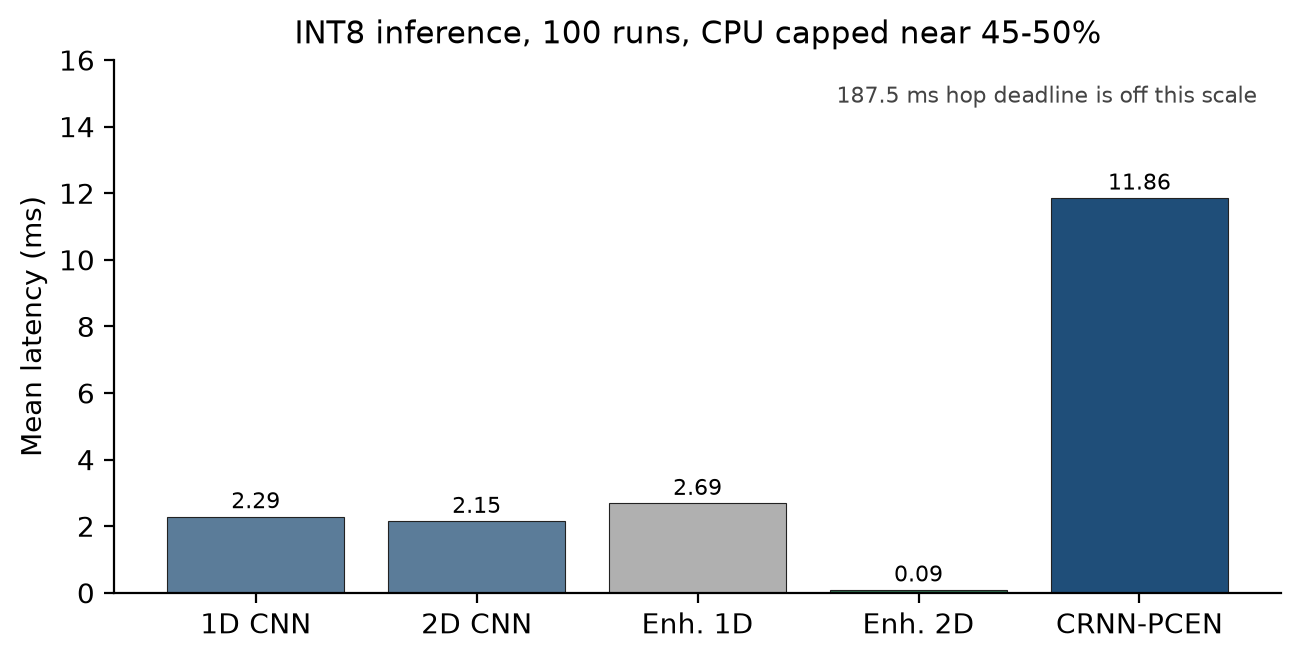
\includegraphics[width=\columnwidth]{figures/fig3_latency.png}
\caption{Mean INT8 inference latency. All models fall well below the 187.5\,ms real-time hop deadline.}
\label{fig:lat}
\end{figure}

\subsection{PCEN Domain Robustness}
To assess microphone invariance, the CRNN-PCEN model was evaluated on both clean audio and synthetically distorted audio (bandpass filtering 150--8{,}000\,Hz, non-linear saturation clipping, additive Gaussian noise at 15--30\,dB SNR, gain perturbation $0.5\times$--$1.5\times$). Sliding-window recall at $\tau=0.50$ was 61\% on both clean and distorted inputs. At $\tau=0.10$, recall was 69\% on both. PCEN's dynamic automatic gain control absorbs transducer-level distortions with zero recall degradation, confirming its utility as a domain-shift normalizer for heterogeneous edge microphones. Imposter rejection improved by 5--7 percentage points under distortion.

\begin{figure}[!t]
\centering
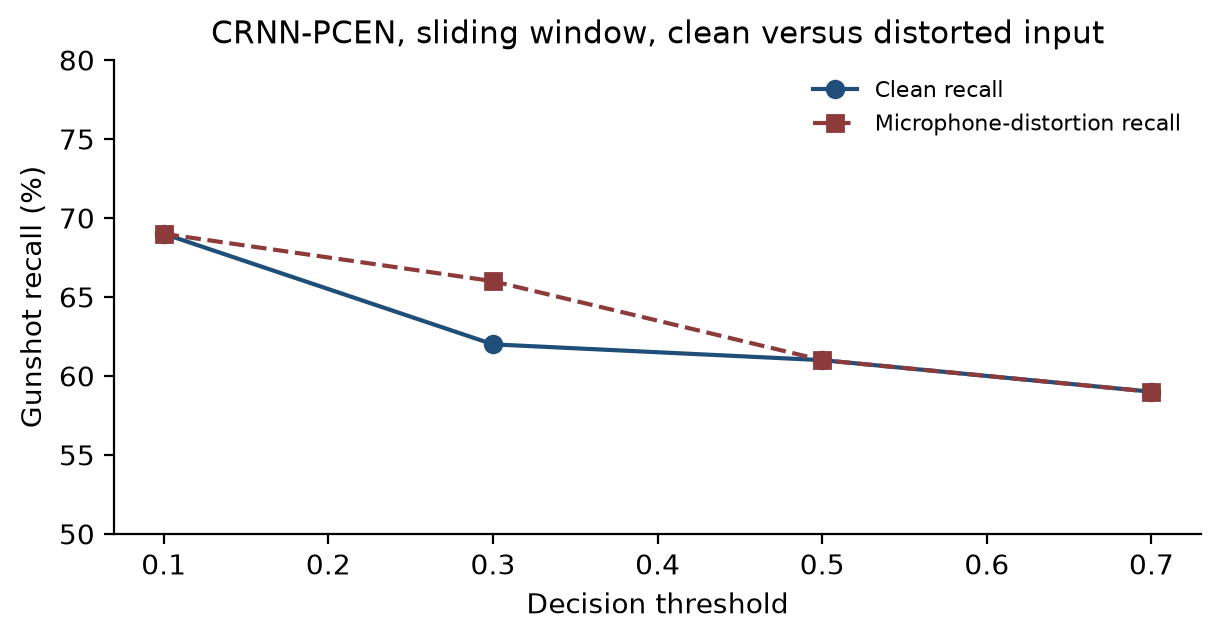
\includegraphics[width=\columnwidth]{figures/fig6_pcen_distortion.png}
\caption{CRNN-PCEN sliding recall under clean versus simulated microphone distortion across multiple decision thresholds.}
\label{fig:pcen}
\end{figure}

\subsection{Multi-Model Ensemble}
\label{sec:ensemble}
An ensemble combining the Enhanced 2D CNN, CRNN-PCEN, and Baseline 1D CNN with adaptive OR-voting was evaluated on the 300-clip benchmark (Table~\ref{tab:ensemble}).

\begin{table}[!t]
\centering
\caption{Ensemble 3-way confusion matrix (300 clips, 100 per class).}
\label{tab:ensemble}
\footnotesize
\begin{tabular}{lcccc}
\toprule
\textbf{True Class} & \textbf{Real} & \textbf{Fake} & \textbf{Not} & \textbf{Acc.} \\
\midrule
Real Gunshot & \textbf{77} & 15 & 8 & 77\% \\
Hard Imposter & 44 & \textbf{46} & 10 & 46\% \\
Ambient & 20 & 38 & \textbf{42} & 80\% \\
\bottomrule
\end{tabular}
\end{table}

\begin{figure}[!t]
\centering
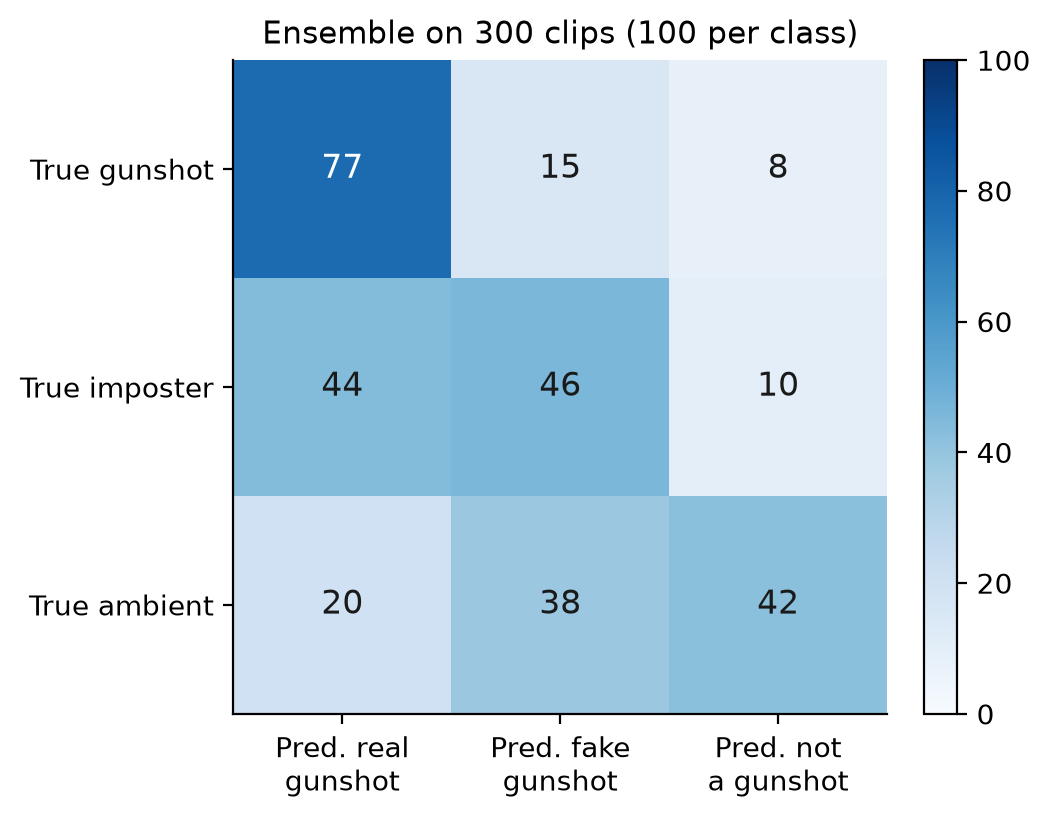
\includegraphics[width=\columnwidth]{figures/fig5_ensemble_confusion.png}
\caption{Ensemble detection counts on 300 clips (100 files per true class).}
\label{fig:cm}
\end{figure}

Ensemble recall reaches 77\% (77/100 gunshots), compared to 67\% for the best single model (sliding). Combined INT8 size is approximately 715\,KB with combined latency of approximately 17\,ms, remaining well within the hop constraint. For resource-constrained single-model deployment, the Enhanced 2D CNN offers the optimal trade-off between recall, specificity, latency, and flash footprint.

\begin{table}[!t]
\centering
\caption{Paradigm comparison summary.}
\label{tab:paradigm}
\footnotesize
\begin{tabular}{lcccc}
\toprule
\textbf{Paradigm} & \textbf{Recall} & \textbf{Spec.} & \textbf{Latency} & \textbf{Flash} \\
\midrule
Peak (single best) & 38\% & 99\% & 0.09\,ms & 124\,KB \\
Sliding (single) & 67\% & 82\% & 0.75\,ms & 124\,KB \\
Multi-model ens. & \textbf{77\%} & 80\% & 17\,ms & 715\,KB \\
\bottomrule
\end{tabular}
\end{table}

% ==============================================================================
\section{Conclusion and Future Work}
\label{sec:conclusion}

This work demonstrates that classical machine learning classifiers achieving near-perfect accuracy on balanced laboratory test sets fail on live microphone input due to temporal feature averaging that destroys impulsive shockwave signatures. The transition from 1D MFCC-based classifiers to 2D spectrogram CNNs---observed both in the Edge Impulse trial and in our TensorFlow models---consistently improved rejection of ambient and imposter sounds. On 300 unseen clips, the Enhanced 2D CNN achieves 67\% gunshot recall (sliding) and 99\% ambient specificity (peak) in 0.09\,ms within 124\,KB. The PCEN-CRNN maintains stable recall under simulated microphone distortion, confirming PCEN as an effective domain-shift normalizer. The Enhanced 1D CNN is not deployable after INT8 conversion due to quantization-induced weight saturation.

A fundamental physical limitation was identified: single-microphone sensing cannot distinguish aerial mortar fireworks from gunfire, as both produce identical shockwave rise-times and reverberation profiles when captured by a single transducer.

The immediate next phase comprises three hardware integration tasks:

\textbf{1) Physical deployment.} Deploy the Enhanced 2D CNN INT8 model on a physical Raspberry Pi~4 to validate virtual machine timing measurements, then port the inference to the Arduino Nano 33 BLE Sense (nRF52840 Cortex-M4F, 1\,MB Flash, 256\,KB SRAM) with its on-board PDM microphone.

\textbf{2) Duty-cycled sleep and one-bit transmission.} The node remains in deep sleep ($\sim$5\,$\mu$A) until a coarse acoustic energy threshold triggers a wake-up. One inference cycle executes, and the node returns to sleep. If the detection score exceeds the threshold, the node transmits a minimal packet containing a node identifier, timestamp, and a single detection bit. If the score is below threshold, no transmission occurs---the radio remains off entirely. Raw audio never leaves the sensor node, ensuring complete privacy. The energy savings from this protocol have not yet been metered.

\textbf{3) Multi-node spatial consensus.} A single sensor node adjacent to a hand clap may occasionally transmit a false detection bit. The gateway raises an alert only when $K \ge 3$ nearby nodes transmit detection bits within the acoustic propagation time window of the deployment site. This spatial consensus eliminates false alarms from localized percussive events. Implementation and testing of this aggregation protocol are planned as the next experimental phase.

\section*{Acknowledgment}
The authors thank Dr. Kaustubh Dhondge for guidance throughout this project. Firearm recordings include the open-access dataset of~\cite{dib2023}. The PCEN front-end follows the formulation of Lostanlen et al.~\cite{lostanlen2019}.

\begin{thebibliography}{4}
\bibitem{dib2023} ``A multi-firearm, multi-orientation audio dataset of gunshots,'' \emph{Data in Brief}, vol.~48, Art. no.~109091, 2023, doi:~10.1016/j.dib.2023.109091.
\bibitem{lostanlen2019} V.~Lostanlen, J.~Salamon, M.~Cartwright, B.~McFee, A.~Farnsworth, S.~Kelling, and J.~P.~Bello, ``Per-channel energy normalization: Why and how,'' \emph{IEEE Signal Process. Lett.}, vol.~26, no.~1, pp.~39--43, 2019.
\bibitem{zhang2018} H.~Zhang, M.~Cisse, Y.~N.~Dauphin, and D.~Lopez-Paz, ``mixup: Beyond empirical risk minimization,'' in \emph{Proc. ICLR}, 2018.
\bibitem{park2019} D.~S.~Park \emph{et al.}, ``SpecAugment: A simple data augmentation method for automatic speech recognition,'' in \emph{Proc. Interspeech}, 2019, pp.~2613--2617.
\end{thebibliography}

\end{document}
